\documentclass[5p,authoryear]{elsarticle}
\makeatletter 
\def\ps@pprintTitle{%
 \let\@oddhead\@empty
 \let\@evenhead\@empty
 \let\@evenfoot\@oddfoot} % Supprimer le bas de page ELSEVIER
\makeatother
\usepackage[utf8]{inputenc} % En unicode
\usepackage[T1]{fontenc}
\usepackage[english]{babel}
\usepackage[babel=true]{csquotes} % permet de faire \enquote{a} (« a »)
\usepackage[fleqn]{amsmath} % pour certains signes mathématiques
\usepackage{amsthm} % Pour \begin{gather}
\usepackage{booktabs} % pour \toprule (un style de tableau)
\usepackage{multirow} % Pour colonnes multiples des tableaux
\usepackage{amssymb} % Pour \leqslant (<=, >=)
\usepackage{float}
\usepackage{hyperref} % DOIT ETRE EN DERNIER
\usepackage[english]{cleveref} % permet de faire \cref au lieu de \ref (DOIT ETRE EN DERNIER)
\usepackage{tikz}
\usepackage{array, longtable, tabularx}% added long table
\usepackage{adjustbox}



\begin{document}

\begin{frontmatter}

\title{Un indicador de seguridad económica para la UE}

\author[1]{Manuel Hidalgo-Pérez\corref{cor1}%
 \fnref{fn1}}
\ead{mhidper@upo.es} 

\author[2]{Jorge Díaz-Lanchas\fnref{fn2}}
\ead{email de jorge}

\author[3]{Miguel Otero\fnref{fn3}}
\ead{email de Miguel}


\cortext[cor1]{Corresponding author}

\affiliation[1]{organization={Universidad Pablo de Olavide},
                addressline={Ctra Utrera s/n},
                postcode={41013},
                city={Sevilla},
                country={España}}

\affiliation[2]{organization={Afiliación Jorge},
                addressline={C. de Mateo Inurria, 25, 27},
                postcode={28036},
                city={Madrid},
                country={España}}

\affiliation[3]{organization={Afiliación Miguel},
                addressline={C. de Mateo Inurria, 25, 27},
                postcode={28036},
                city={Madrid},
                country={España}}


\begin{abstract}
Musho Beti
\end{abstract}

\begin{keyword}
XXXX \sep XXXX \sep XXX \sep XXX \\
\textbf{JEL Codes:} XX, XX, XX
\end{keyword}

\end{frontmatter}

\section{Introducción}

\section{Metodología. Indicador de dependencia}

\subsection{Dependencia del país $E$}

Asumamos que queremos medir la dependencia de un país $i$ de las importaciones de un país tercero ($E$). El objetivo es valorar hasta qué punto el país $i$ está sujeto a los posibles riesgos de depender en exceso para una industria o bien de dicho país. Una primera opción sería la de calcular el porcentaje que representan las importaciones a este país $i$ desde $E$ del bien. En el numerador se incluiría el total importado desde $E$ mientras que en el denominador se sumarían todas las importaciones desde cualquier país así como la producción interna.

Este indicador es el que, entre otros, publica el Banco Central Europeo (ECB, 2023). Formalmente:

\begin{equation}
    CD2_{iE} = \frac{M_{iE}}{\sum_{j} M_{ij} + P_i}
\end{equation}

donde:
\begin{itemize}
    \item $M_{iE}$ representa las importaciones del país $i$ desde el país $E$
    \item $M_{ij}$ son las importaciones del país $i$ desde cualquier país $j$
    \item $P_i$ es la producción interna del país $i$
\end{itemize}

Aunque en realidad el ECB calcula tres indicadores diferentes, uno de ellos, el CD2, llamado de dependencia, cuantifica el porcentaje descrito anteriormente. 

Sin embargo, esta medición adolece de una limitación importante. El uso del porcentaje de las disponibilidades totales de un bien como medida de la dependencia pasa por alto que, en entornos comerciales globalizados e integrados, parte de dicha dependencia puede establecerse a través de otros países con los que se tengan vínculos comerciales estrechos. Así, la posible existencia de "hubs" comerciales en algunos países puede "trasladar" hacia otros países posibles dependencias que mediante el indicador publicado por el ECB (2023) no sería posible medir.

Así, podemos pensar que a la dependencia de $i$ de las importaciones de $E$ medidas como se ha indicado arriba, y que podemos denominar dependencia directa, puede existir otra indirecta, y que corresponde a la dependencia que de $E$ tiene $i$ a través de un país $j$ porque, a su vez, este último posea su respectiva dependencia. La figura 1 dibuja esta posible dicotomía, de dependencia directa e indirecta, definiendo a $1$ como nuestro país de referencia, a $E$ el país sobre el que queremos medir la dependencia y $2$ un posible socio comercial de $1$ que a su vez depende de $E$ y que traslada dicha dependencia a $1$ de forma indirecta.

\begin{figure}[h]
    \begin{center}
        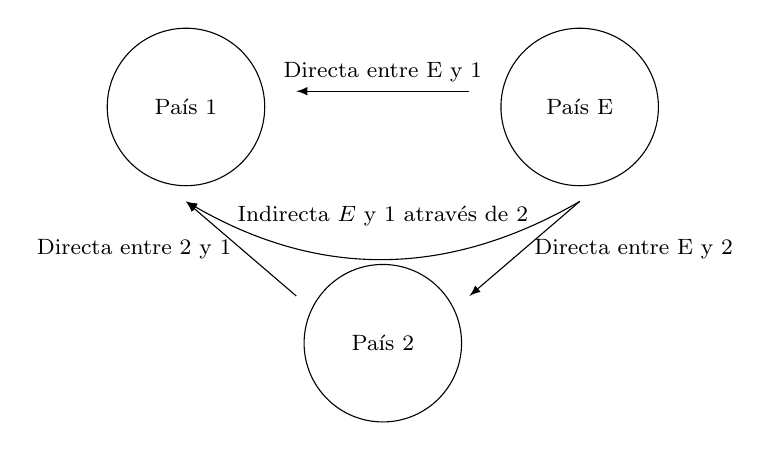
\begin{tikzpicture}[font=\footnotesize]]
                    % Círculos
                    \draw (0,0) circle (1cm) node {País 1};
                    \draw (5,0) circle (1cm) node {País E};
                    \draw (2.5,-3) circle (1cm) node {País 2};
                
                    % Flechas
                    \draw [-latex, >=latex] (3.6,0.2) -- (1.4,0.2) node [midway,above] {Directa entre E y 1};
                    \draw [-latex, >=latex] (5,-1.2) -- (3.6,-2.4) node [midway,right] {Directa entre E y 2};
                    \draw [-latex, >=latex] (1.4,-2.4) -- (0,-1.2) node [midway,left] {Directa entre 2 y 1};
            
                    % Flecha curva
                    \draw [-latex, >=latex, bend left] (5,-1.2) to node[above=0.3cm, midway] {Indirecta $E$ y $1$ através de $2$} (0,-1.2);
        \end{tikzpicture}
        \caption{Diagrama de flujo entre países.}
        \label{fig:flujo-paises}
    \end{center}
\end{figure}

En la figura, cada nodo representa un país y las aristas o flechas representan la existencia de flujos comerciales. Obviamente, en cada caso, dichos flujos pueden ser en ambas direcciones, pero por simplicidad se han dibujado aquellos que son relevantes para la explicación.

Así, la dependencia de $1$ respecto de $E$ vendría por la suma de las dependencias directas, que se corresponde con el flujo superior del diagrama, y de la indirecta que proveniene de $E$ y que cruza hasta $1$ a través de $2$. Sin embargo, esta dependencia indirecta no se quedaría solamente en el flujo dibujado bajo tal nombre en la figura \ref{fig:flujo-paises}. podría suceder que, habiendo un país tercero, la depoendencia indirecta ya no solo podría llegar a $1$ desde $3$, sino que udiera hacerlo desde $2$ por susimportaciones desde $3$ y estas desde $E$. Dicho de otro modo, la dependencia indirecta correspondería a la suma de todos los flujos comerciales, definidos como todas las opciones posibles de caminos alternativos que, partiendo desde $E$ lleguen a $1$. Aunue estos caminos son limitados en el caso de tres países, cuando disponemos de más de dos centenares de países, el cálculo se complica. Sin embargo, dicha complicación no significa que sea imposible llevar a cabo tal computación. 

\subsection{Cálculo de Dependencias Indirectas}
\subsubsection{Formulación Matricial Base}

Para formalizar el cálculo de dependencias indirectas, consideremos un sistema de $n+1$ países, donde $n$ países forman el conjunto $\Omega = \{1,2,3\}$ y un país externo $E$. La matriz de flujos comerciales se define como:

\begin{equation}
    X =
    \begin{bmatrix}
    x_{11} & x_{12} & x_{13} & x_{1E} \\
    x_{21} & x_{22} & x_{23} & x_{2E} \\
    x_{31} & x_{32} & x_{33} & x_{3E} \\
    x_{E1} & x_{E2} & x_{E3} & x_{EE}
    \end{bmatrix}
\end{equation}

donde $x_{ij}$ representa las importaciones del país $i$ desde el país $j$.

\subsubsection{Dependencias Directas}
La dependencia directa (nivel 1) del país $i$ respecto a $E$ se define como:

\begin{equation}
    \delta_i^1 = a_{Ei} = \frac{x_{Ei}}{\sum_{j} x_{ji} + x_{ii}}
\end{equation}

Esta medida coincide con el indicador CD2 del BCE pero representa solo el primer nivel de dependencia.

\subsubsection{Dependencias por Niveles}

La dependencia de nivel 2 para el país 1 incorpora efectos indirectos a través de países intermediarios:

\begin{equation}
    \delta_1^2 = a_{21}a_{E2} + a_{31}a_{E3}
\end{equation}

Generalizando para todos los países en $\Omega$:

\begin{equation}
    \delta^2 = a_E A_\Omega
\end{equation}

donde $a_E = [a_{E1} \quad a_{E2} \quad a_{E3}]$ y $A_\Omega$ es la matriz de dependencias directas con diagonal nula:

\begin{equation}
    A_\Omega =
    \begin{bmatrix}
    0 & a_{12} & a_{13} \\
    a_{21} & 0 & a_{23} \\
    a_{31} & a_{32} & 0
    \end{bmatrix}
\end{equation}

\subsubsection{Dependencia Total mediante Series de Leontief}

La dependencia total incorpora efectos de todos los niveles:

\begin{align}
    \delta &= \delta^1 + \delta^2 + \delta^3 + \cdots \\
    &= a_E + a_E A_\Omega + a_E A_\Omega^2 + \cdots \\
    &= a_E(I + A_\Omega + A_\Omega^2 + \cdots) \\
    &= a_E(I - A_\Omega)^{-1}
\end{align}

Esta formulación, implementada en el método \texttt{calcular\_dependencia\_total}, captura:
\begin{itemize}
    \item Dependencias directas ($\delta^1$)
    \item Efectos de primer orden ($\delta^2$)
    \item Efectos de segundo orden ($\delta^3$)
    \item Todos los efectos de orden superior
\end{itemize}

\subsubsection{Interpretación como Grafo Dirigido}
La metodología puede interpretarse como un análisis sobre un grafo dirigido ponderado donde:
\begin{itemize}
    \item Los nodos representan países
    \item Las aristas representan flujos comerciales
    \item Los pesos son los coeficientes $a_{ij}$
    \item Los caminos de longitud $k$ corresponden a dependencias de nivel $k$
\end{itemize}

La matriz $(I - A_\Omega)^{-1}$ captura todos los posibles caminos en el grafo, proporcionando una medida completa de la dependencia total.

\subsection{Extensión del Modelo: Análisis con Dos Países Externos}

La metodología puede extenderse para analizar dependencias respecto a dos países externos simultáneamente ($E_1$ y $E_2$). Esta extensión es particularmente relevante cuando las cadenas de dependencia pueden establecerse a través de múltiples países externos al conjunto $\Omega$.

\subsubsection{Formulación Matricial Extendida}

Para cada país externo $E_k$ ($k \in \{1,2\}$), definimos:

\begin{equation}
    A_k =
    \begin{bmatrix}
    a_{11}^k & a_{12}^k & \cdots & a_{1E_k} \\
    a_{21}^k & a_{22}^k & \cdots & a_{2E_k} \\
    \vdots & \vdots & \ddots & \vdots \\
    a_{E_k1} & a_{E_k2} & \cdots & a_{E_kE_k}
    \end{bmatrix}
\end{equation}

Las matrices $A_{\Omega_k}$ se construyen incluyendo el país externo complementario:
\begin{equation}
    A_{\Omega_k} = A_k|_{\Omega \cup \{E_{3-k}\}}
\end{equation}

\subsubsection{Cálculo de Dependencias por Niveles}

1. Dependencias Directas (Nivel 1):
\begin{align}
    \delta_1^1 &= a_{E_1} \\
    \delta_2^1 &= a_{E_2}
\end{align}

2. Dependencias Indirectas (Nivel 2):
\begin{align}
    \delta_1^2 &= a_{E_1}A_{\Omega_1} \\
    \delta_2^2 &= a_{E_2}A_{\Omega_2}
\end{align}

3. Dependencias de Nivel Superior:
Para cualquier nivel $p > 2$:
\begin{align}
    \delta_1^p &= a_{E_1}A_{\Omega_1}^{p-1} \\
    \delta_2^p &= a_{E_2}A_{\Omega_2}^{p-1}
\end{align}

\subsubsection{Dependencia Total}

La dependencia total para cada país externo se obtiene mediante la suma de series infinitas:

\begin{equation}
    \delta_k = \sum_{p=1}^{\infty} \delta_k^p = a_{E_k}[I - A_{\Omega_k}]^{-1}, \quad k \in \{1,2\}
\end{equation}

\subsubsection{Propiedades del Sistema Dual}

El sistema con dos países externos presenta propiedades específicas:

1. Interacción entre Dependencias:
   \begin{itemize}
       \item Las dependencias de $E_1$ pueden verse afectadas por la presencia de $E_2$
       \item Los efectos indirectos pueden transmitirse a través de ambos países externos
   \end{itemize}

2. Matrices de Transición:
   \begin{itemize}
       \item $A_{\Omega_1}$ captura transiciones incluyendo $E_2$
       \item $A_{\Omega_2}$ captura transiciones incluyendo $E_1$
   \end{itemize}

3. Interpretación en Teoría de Grafos:
   \begin{itemize}
       \item Los caminos pueden incluir nodos de ambos países externos
       \item La conectividad del grafo aumenta con la inclusión del segundo país externo
   \end{itemize}

Esta extensión del modelo permite un análisis más completo de las interdependencias en sistemas comerciales complejos donde múltiples países externos pueden ejercer influencia simultánea sobre el conjunto $\Omega$.



\subsection{Concentración de la dependencia}

Un segundo indicador que podría complementar la visión sobre la dependencia de un país de las importaciones de terceros países sería el indicador de concentración de dicha dependencia. En pocas palabras, no solo es relevante depender de países externos para la disponibilidad de los bienes consumidos de una determinada industria, sino que también es relevante considerar si esa dependencia está concentrada en pocos países.

El indicador natural en este caso es el cálculo de un índice de Herfindahl. Así, si $s_{ij}$ es un indicador de dependencia que varía entre 0 y 1 en lugar de ser el porcentaje de participación en el mercado, podemos reinterpretar el índice de Herfindahl de la siguiente manera:


\[ H_j = \sum_{i=1}^{n} s_{ij}^2 \],

donde

$H$ es el índice de Herfindahl, $n$ es el número de países sobre los que calculamos el índice de dependencia en la industria j y $s_{ij}$  representa el indicador de dependencia del país $i$ en la industria $j$.
    
El índice de Herfindahl, calculado de esta manera, proporcionaría una medida de la concentración de la dependencia en la industria o sector en cuestión. Un valor más cercano a 1 indicaría una alta concentración de dependencia en unos pocos países, mientras que un valor más cercano a 0 indicaría una distribución más equitativa de la dependencia entre los diferentes países.


\section{Descripción de la base de datos}
(Jorge)


\section{Resultados: un ejemplo para España}

En esta sección se presentan los resultados del cálculo de la dependencia para España. Para ello, es necesario calcular la dependencia para cada una de las industrias con información disponible sobre importaciones, así como los países de origen, utilizando la fórmula representada en (\ref{eq: total}).

La Tabla \ref{tab:mi_tabla} muestra los veinte productos con mayor dependencia y concentración. Destacan "Manufacturing services on physical inputs owned by others", "Animal feed ingredients and pet foods", "Processing of nuclear fuel" y "Electricity distribution & control apparatus".

La construcción del índice proporciona información sobre los países de origen de las dependencias. Por ejemplo, para el primer servicio mencionado, la dependencia se concentra principalmente en China, Gran Bretaña y Estados Unidos, ya que estos tres países representan un total de 1.62 puntos de los 2.85, dejando el resto de la dependencia para otros países. Esta concentración determina que estos servicios no solo tengan una alta dependencia, sino también una alta concentración.

En el caso del "Processing of nuclear fuel", la dependencia, que también es alta, se concentra en Gran Bretaña, Rusia, Estados Unidos, Canadá y Kazajstán. Entre estos cinco países, se obtienen 1.95 puntos de los 2.23 correspondientes al valor total de dependencia. Sin embargo, la distribución más o menos equitativa de esta dependencia entre estos cinco países resulta en una concentración algo menor (ver Figura \ref{fig:fig1}).


\begin{figure*}[t] % Utilizamos figure* en lugar de figure
    \centering
    \caption{Bandwith optimal selection}
    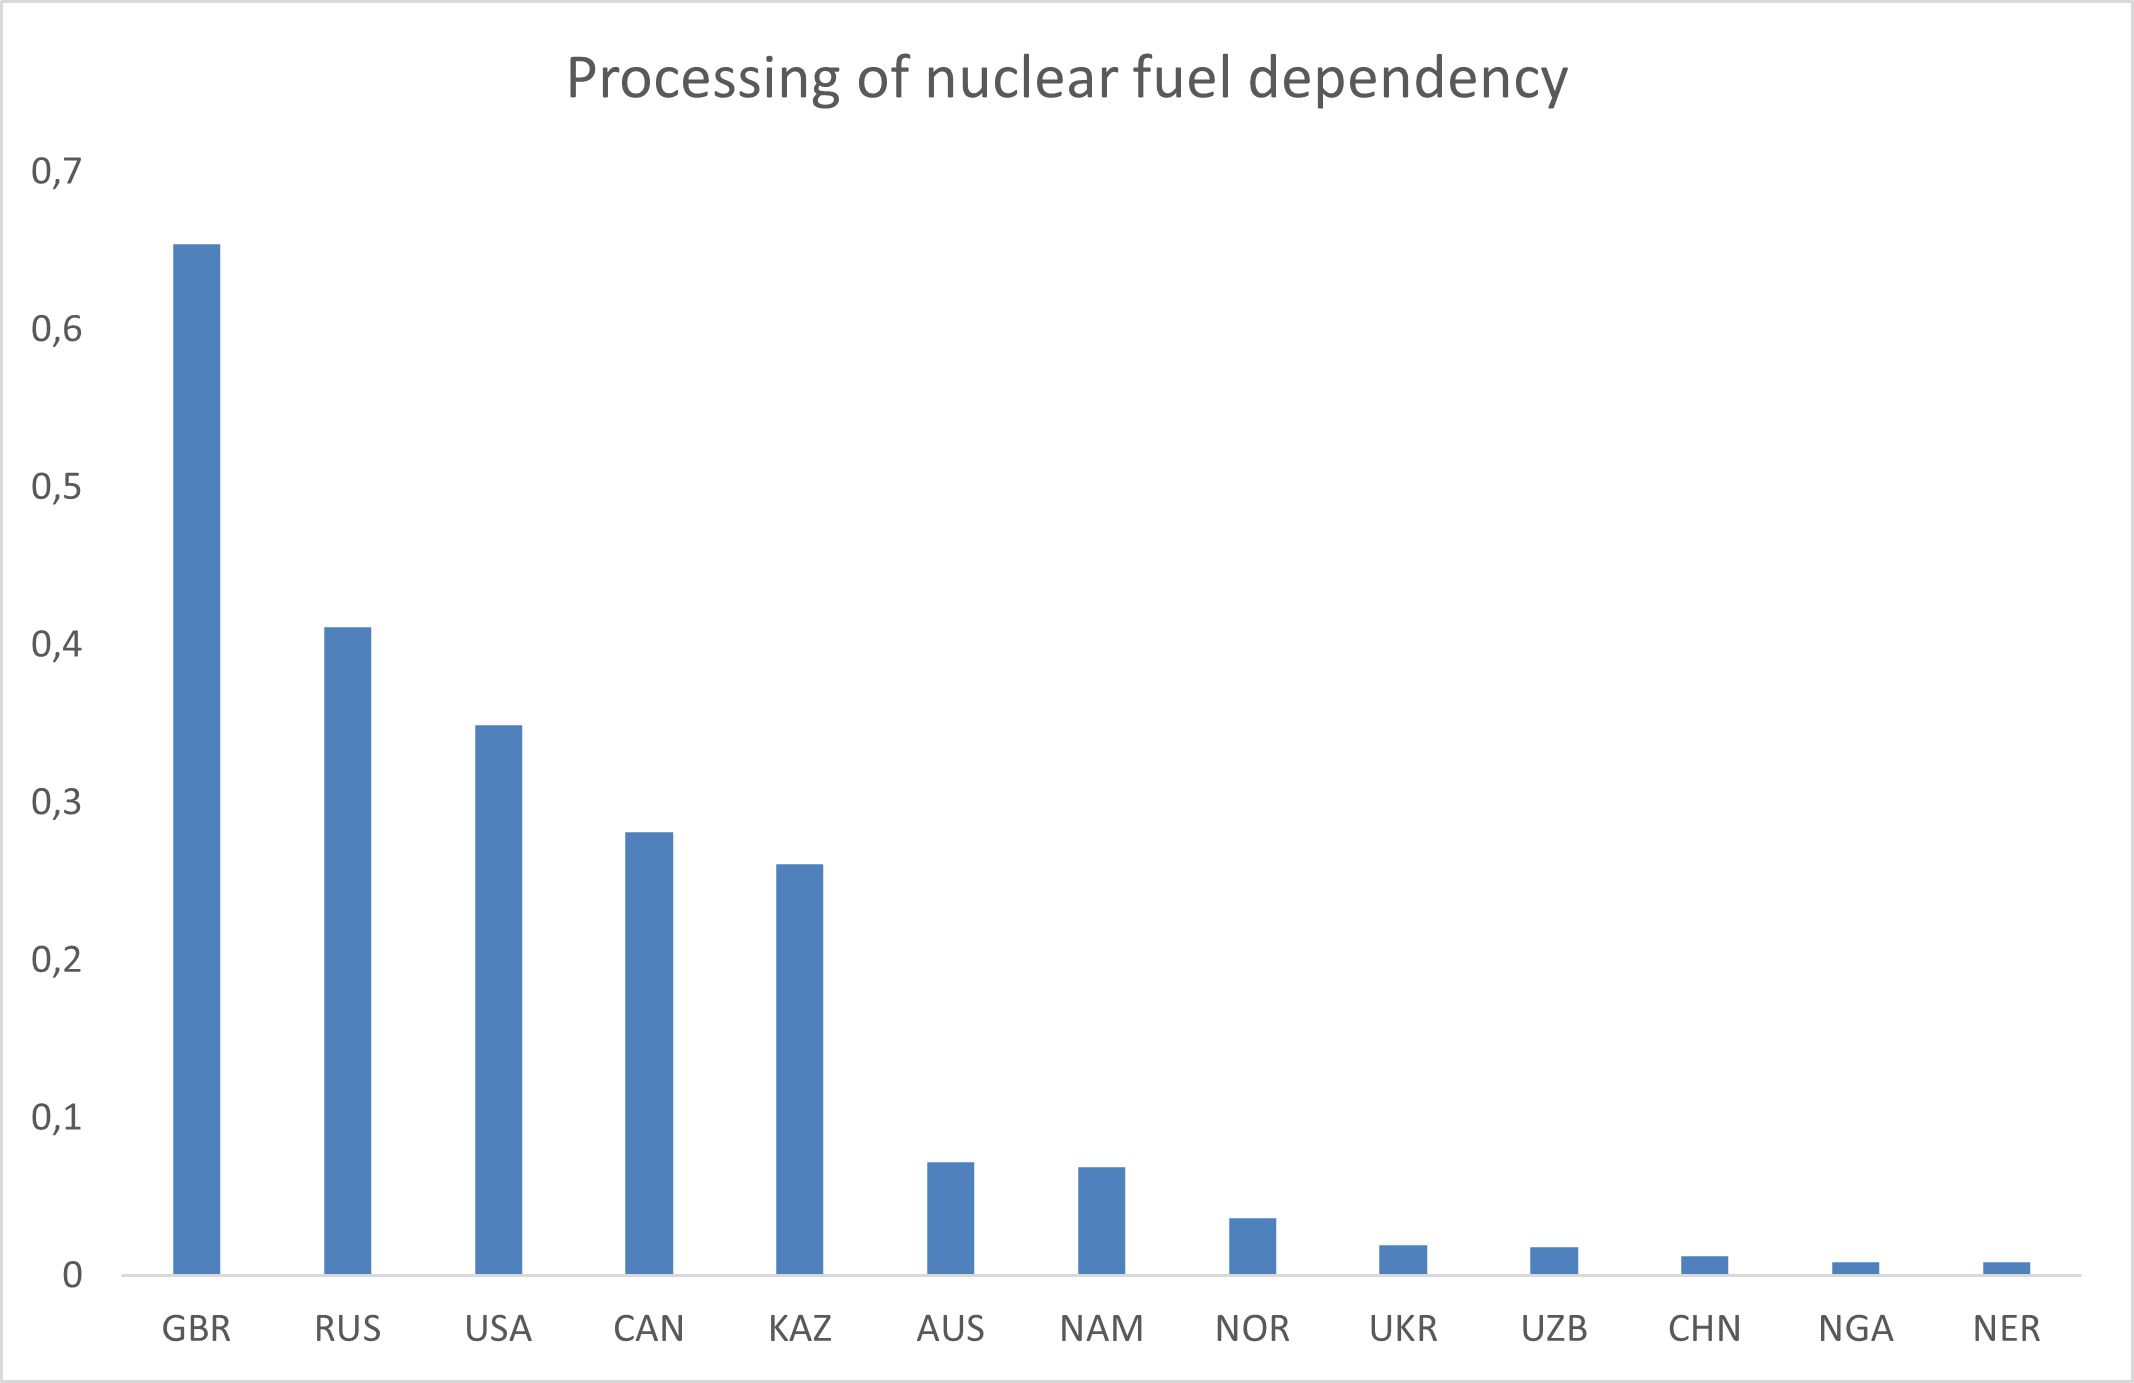
\includegraphics[width=0.7\linewidth]{../Imagenes/Nuclear fig.png}
    \label{fig:fig1}
\end{figure*}

Dado que el resultado en todos los casos sería de una matriz para cada país, las posibilidades de moestrar resultados y figuras así como análkisis complementarios resultaría interesante. 

\subsection{Agregación de dependencia y concentración}

Finalmente, queda por describir la síntesis de ambos indicadores, de concentración y depedencia en uno solo. Este paso, pretende ser lo más objetivo posible, tratando de evitar la definicion de funciones o pesos arbitrarios por parte de los autores. 
Así, para justificar nuestra decisión el primer paso es visualizar 


\begin{figure*}[t] % Utilizamos figure* en lugar de figure
    \centering
    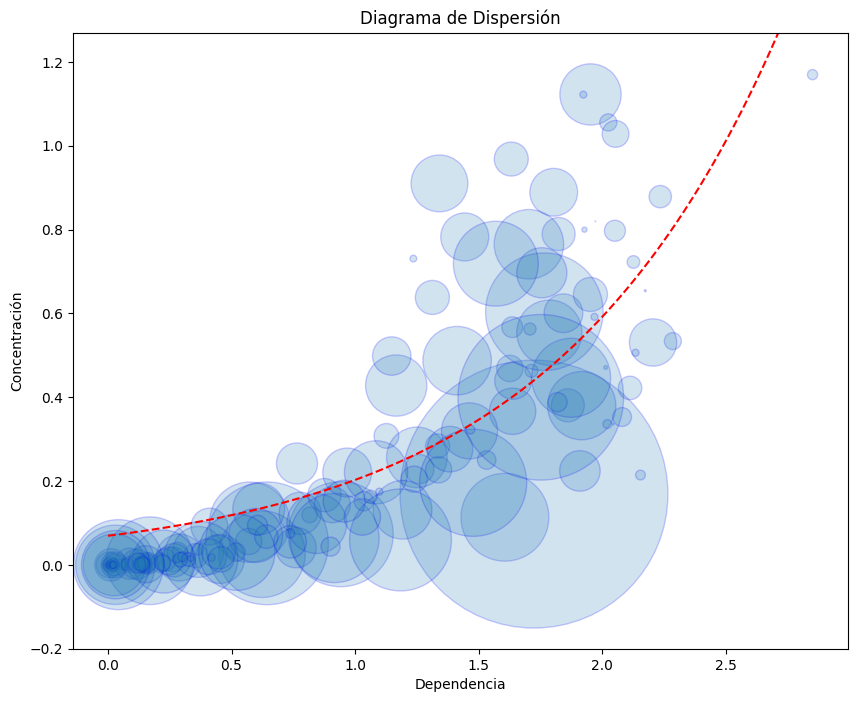
\includegraphics[width=0.8\linewidth]{../Imagenes/scatter.png}
    \caption{Descripción del gráfico 1.}
    \label{fig:fig2}
\end{figure*}


    
\begin{table*}{c|c|c}
\caption{Descripción de tu tabla}
\begin{center}
\label{tab:mi_tabla}
\begin{tabular}{lrr}
\hline

\hline
                                                           &   dependencia &         hfd \\
\hline
 Manufacturing services on physical inputs owned by others &   2.85162     & 1.1698      \\
 Animal feed ingredients and pet foods                     &   2.28618     & 0.533954    \\
 Processing of nuclear fuel                                &   2.23532     & 0.878671    \\
 Electricity distribution \& control apparatus              &   2.20599     & 0.530653    \\
 Live Cattle                                               &   2.17455     & 0.65423     \\
 Forestry                                                  &   2.15508     & 0.214409    \\
 Other meats, livestock products, and live animals         &   2.13504     & 0.506171    \\
 Other publishing                                          &   2.12676     & 0.722794    \\
 Jewellery and related articles                            &   2.11297     & 0.422262    \\
 Fishing                                                   &   2.08054     & 0.352859    \\
 Maintenance and repair services n.i.e.                    &   2.05423     & 1.02829     \\
 Publishing of books and other publications                &   2.05168     & 0.797229    \\
 Cereal products                                           &   2.04503     & 0.335872    \\
 Government goods and services n.i.e.                      &   2.02493     & 1.05569     \\
 Tobacco leaves and cigarettes                             &   2.02105     & 0.33592     \\
 Cotton                                                    &   2.0143      & 0.471187    \\
 Live Swine                                                &   1.97258     & 0.819729    \\
 Prepared fruits and fruit juices                          &   1.96906     & 0.591794    \\
 Charges for the use of intellectual property n.i.e.       &   1.95293     & 1.1225      \\
 Optical instruments \& photographic equipment              &   1.95268     & 0.645241    \\
 Dressing \& dyeing of fur; processing of fur               &   1.92843     & 0.799905    \\
 Publishing of newspapers journals etc.                    &   1.9239      & 1.1221      \\
 Other chemical products n.e.c.                            &   1.91718     & 0.379988    \\
 Other agricultural products, nec                          &   1.90995     & 0.224258    \\
 Other electrical equipment n.e.c.                         &   1.87459     & 0.446511    \\
 Beverages, nec                                            &   1.86125     & 0.380674    \\
 Mining of hard coal                                       &   1.84339     & 0.600476    \\
 Mining of iron ores                                       &   1.82385     & 0.789468    \\
 Spices                                                    &   1.8195      & 0.388195    \\
 Luggage handbags etc.; saddlery \& harness                 &   1.80408     & 0.889134    \\

\hline
\end{tabular}
\end{center}
\end{table*}

\newpage
\appendix
\section{Algoritmo de computación de las dependencias}

En este apartado, describimos el algoritmo implementado y las funciones utilizadas para analizar la dependencia comercial entre países. El algoritmo consta de varias etapas que se detallan a continuación.

\subsection{Crear matriz de comercio}

La función \texttt{crear\_matriz\_comercio} toma como entrada un conjunto de datos agrupados por industria y genera una matriz de comercio para cada industria. Para ello, inicializa una matriz vacía para cada industria y luego llena esta matriz con los valores de comercio correspondientes.

\subsection{Calcular vectores AE y matrices normalizadas}

La función \texttt{calcular\_vectores\_ae} calcula los vectores de efecto autárquico (AE) y las matrices normalizadas para cada industria. Primero, normaliza cada matriz de comercio dividiendo cada celda por la suma de su columna correspondiente. Luego, extrae el último vector de cada matriz normalizada, que representa el efecto autárquico.

\subsection{Obtener submatrices}

La función \texttt{obtener\_submatrices} toma las matrices normalizadas y genera submatrices excluyendo la última fila y columna de cada una. Estas submatrices se utilizan posteriormente para calcular las matrices inversas.

\subsection{Calcular matrices inversas}

La función \texttt{calcular\_matrices\_inversas} calcula las matrices inversas para cada submatriz obtenida en la etapa anterior. Para ello, resta la matriz identidad de la submatriz normalizada y calcula la inversa de la matriz resultante.

\subsection{Calcular dependencia}

Finalmente, la función \texttt{calcular\_dependencia} calcula la dependencia comercial entre países utilizando los vectores AE y las matrices inversas calculadas. Multiplica cada vector AE por la matriz inversa correspondiente y almacena el resultado en un DataFrame, donde las filas representan las industrias y las columnas representan los países. 

\end{document}

